\documentclass[10pt]{article}
\usepackage[margin=0.72in]{geometry}
\usepackage{booktabs,graphicx,array,microtype,xcolor,listings,caption,subcaption,xspace}
\usepackage[section]{placeins}
\usepackage[numbers,sort&compress]{natbib}
\usepackage[hidelinks]{hyperref}
\usepackage[nameinlink,noabbrev]{cleveref}
\graphicspath{{figures/}}
\definecolor{shade}{gray}{0.94}
\lstset{basicstyle=\ttfamily\footnotesize,backgroundcolor=\color{shade},frame=single,columns=fullflexible,breaklines=true}
\newcommand{\us}{\ensuremath{\mu\mathrm{s}}\xspace}
\newcommand{\eclass}[1]{\textsc{#1}}
\title{A Change of Core:\\Revisiting ESP32 Benchmarks on ESP32-C6}
\author{Izbassar Yesbol\\[-0.2em]\small\href{mailto:hello@izba.sarl}{hello@izba.sarl}\\\small ORCID: \href{https://orcid.org/0009-0002-1737-7982}{0009-0002-1737-7982}}
\date{Technical report, editorial revision 1.0.1, October 2026}

\begin{document}
\maketitle
\begin{abstract}
Plauska et al.'s classic-ESP32 benchmarks offer a way to revisit familiar workloads on ESP32-C6, whose processor uses RISC-V rather than Xtensa. We measured CRC-32, SHA-256, Q15 FFT, binary32 FIR, and binary32 IIR in C/C++, Rust, and MicroPython on one C6 board. Correctness-gated runs produced 12,000 reproduction-oriented observations and 9,600 observations under declared performance transformations. Historical aggregates provide a descriptive comparator; exact C6 binaries and matched, unmeasured Xtensa and RV32IMAC reconstructions provide separate generated-code evidence.

At the largest input, local native CRC-32, SHA-256, and FFT means were lower than the published means, while FIR and IIR means were higher. Within C6, the C++ and Rust ordering changed by workload. MicroPython was 22--890$\times$ slower than C++ locally, although its local means were below the historical means for all five workloads. C6 FIR/IIR binaries call software floating-point helpers, whereas matched Xtensa objects emit floating-point instructions. An audited Rust FFT transformation reduced the median by 22.7\% relative to its safe performance build while changing the whole kernel. The C6 SHA peripheral reduced the Mode A software time by a factor of 8.70.

Software floating point is a plausible contributor to the FIR/IIR contrast, but these measurements cannot quantify its contribution. Hardware, toolchain, runtime, and protocol differences also prevent an ISA-only interpretation of this single-board case study.
\end{abstract}

\section{Introduction}
Moving a benchmark from classic ESP32 to ESP32-C6 changes more than the instruction set. The former integrates Xtensa LX6 cores; the latter uses an Espressif RISC-V core configured as RV32IMAC \citep{espressifESP32Datasheet,espressifESP32C6Datasheet}. Caches, flash, board, compiler backend, SDK, runtime, and protocol may change too. Throughout this paper, \emph{platform} denotes that complete context, \emph{ISA} the instruction-set contract, \emph{target} a compiler configuration, and \emph{generated code} a particular artifact.

Plauska et al. measured C/C++, Rust, MicroPython, and TinyGo on classic ESP32 using five kernels \citep{plauska2023performance}. We revisit those workloads in the first three languages on C6. Recovering the historical protocol required resolving differences in warm-ups, launchers, and MicroPython timing boundaries; some input and acquisition details remain incomplete. All comparisons with Plauska are therefore \emph{historical and descriptive}. Only the C6 was newly measured. Our matched Xtensa objects show how pinned toolchains compile the recovered source; they neither reproduce Plauska's binaries nor supply Xtensa timing.

The resulting dataset contains 21,600 observations under common C6 timing rules, with provenance and correctness checks. We use exact C6 artifacts and matched Xtensa/RV32IMAC reconstructions to examine the code behind the results. A separate optimization campaign tests compiler profiles, a Rust safety transformation, and the SHA peripheral without changing the reproduction-oriented baseline.

\section{Architecture and Evidence}
The decomposition of execution time into dynamic instruction count, cycles per instruction, and clock rate helps distinguish what a benchmark measures from what might explain it \citep{hennessy2025quantitative,patterson2020cod}. Here we measure elapsed kernel time. Dynamic count, CPI, cache misses, and stalls remain unmeasured, and we do not derive cycles from nominal frequency. Disassembly reveals which instructions were emitted, but not how often they execute or how much time they consume.

RISC-V's open instruction-set contract \citep{asanovic2014free,patterson2017reader} and Xtensa's configurable design \citep{gonzalez2000xtensa} both require attention to the implemented target. A generic Xtensa manual \citep{cadenceXtensaISASummary} does not establish which optional features a particular ESP32 contains.

The classic ESP32 datasheet identifies LX6 processors with floating-point support (\S4.1.1) \citep{espressifESP32Datasheet,espressifESP32TRM}. The C6 datasheet specifies RV32IMAC (\S4.1.1.1); its technical reference manual sets the standard single-precision extension bit to zero (\texttt{misa}, register 1.6, p.~45) \citep{espressifESP32C6Datasheet,espressifESP32C6TRM}. We use the unprivileged specification for RISC-V instruction semantics \citep{riscvUnpriv2026} and the preserved binaries to establish what each compiler emitted.

For each kernel, we inspect its numeric representation, loop, surrounding memory and control operations, and any checks or helper calls that survive compilation. \Cref{tab:evidence} identifies the evidence available for interpreting those observations.

\begin{table}[!htbp]
\centering\small
\caption{Evidence classes keep observations separate from interpretations.}
\label{tab:evidence}
\begin{tabular}{@{}p{0.17\linewidth}p{0.72\linewidth}@{}}
\toprule Class & Meaning \\ \midrule
\eclass{Measured} & Physical C6 timing and exact preserved C6 build evidence.\\
\eclass{Published} & Plauska aggregate values; never expanded into synthetic samples.\\
\eclass{Reconstructed} & Matched-source Xtensa/RV32IMAC static artifacts; not executed.\\
\eclass{Documented} & Vendor, ISA, ABI, or toolchain statements.\\
\eclass{Derived} & Reproducibly computed summaries, ratios, tables, and figures.\\
\eclass{Inferred} & Mechanism explanation bounded by the preceding evidence.\\
\bottomrule
\end{tabular}
\end{table}

\section{Related Work}
Plauska et al. supply the five workloads and the published classic-ESP32 baseline used here \citep{plauska2023performance}. Ionescu and Enescu compare C and MicroPython on ESP32 and STM32 \citep{ionescu2020micropythonc}; Tan et al. examine scripting runtimes on ESP32 \citep{tan2025scripting}; and Tan and Hakala evaluate event-driven statecharts and MicroPython on ESP32-C3 \citep{tan2026eventdriven}. Their workload and runtime contracts differ from the five kernels reconstructed here.

Two studies overlap more directly with the platform question. Molano Rodr\'iguez measures classic ESP32 and ESP32-C6 with Dhrystone implementations adapted separately per platform, and attributes the higher C6 score to the RISC-V architecture alongside internal SoC optimisations \citep{molano2025riscvfpga}. Embuena et al. compare C and Rust across classic ESP32, ESP32-C3, and Arm boards, measuring execution time and energy for sorting, FIR, PID, and state-machine workloads \citep{embuena2026platforms}. Neither study reconstructs Plauska's five-workload protocol on C6, and neither combines its three retained languages with the matched code artifacts reported here; the per-platform adaptation the Dhrystone comparison required also limits what its contrast identifies. We therefore claim neither the first physical ESP32/C6 comparison nor the first cross-architecture language comparison.

Ariel OS addresses embedded Rust across heterogeneous targets \citep{frank2025ariel}, and Femto-Containers studies portable isolation across microcontrollers \citep{zandberg2022femtocontainers}. Lima examines cryptographic performance, energy, and memory on C6 \citep{lima2025esp32c6signatures}; Has et al. include C6 in an evaluation of constrained WebAssembly runtimes \citep{has2025wasmiot}. These are adjacent questions: the present measurements cover kernel time and generated code, with no energy, scheduling, or virtual-machine experiment.

Trancă et al. compare twelve scalar C workloads on classic ESP32, RP2040, and STM32F446 under maximum-clock and common-160-MHz profiles, measuring latency and active-computation energy \citep{tranca2026workload}. Their common-frequency comparison retains board and software differences. It complements the present study's focus on C6, three languages, and generated code.

\section{Research Questions and Scope}
\textbf{RQ1.} How does generated code differ between exact measured C6 RV32IMAC artifacts and matched reconstructed Xtensa artifacts? Which documented target mechanisms are consistent with the local measurements and the direction of the historical comparison?

\textbf{RQ2.} Under a reconstructed common protocol, how do C/C++, Rust, and MicroPython compare within the measured C6, and how do those local results differ descriptively from Plauska's aggregates?

Mode B asks how each native language's declared performance profile changes local timing, and what the dedicated C6 SHA peripheral changes relative to frozen software. It does not equate optimizer levels or call hardware SHA an ISA feature.

\section{Methodology}
\subsection{Design, board, and controls}
This is a single-board C6 case study plus historical comparison and matched static-code analysis. The physical target was one ESP32-C6 revision 0.2 module on an ESP32-C6 Relay X1 carrier with 4 MB DIO flash at 80 MHz. The high-performance CPU was fixed and read back at 160 MHz. Dynamic frequency scaling, sleep, Wi-Fi, BLE, and IEEE 802.15.4 were disabled. Supply, ambient conditions, between-day variability, and board-unit variability were not controlled. Energy was not measured.

Native timing uses \texttt{esp\_timer\_get\_time()}; MicroPython uses \texttt{time.ticks\_us()}. A resolution pilot selected repeated-kernel batches for short calls. Every raw row retains batch count, total duration, and normalized per-call time. Serial output, allocation, slicing/copying, table construction, GC preparation, validation, and cleanup lie outside the timed kernel. Small inputs principally reveal fixed/timer overhead and are not treated as throughput.

\subsection{Mode A contract}
Mode A reconstructs the historical workloads under common C6 rules. Each language uses the same recovered algorithm, canonical input, eight sizes (0, 16, 32, 64, 128, 256, 512, and 1024 workload units), correctness requirements, one unmeasured warm-up, and 100 accepted observations per size. CRC is CRC-32/ISO-HDLC; SHA is frozen software SHA-256; FFT preserves Q15 complex representation and scaling; FIR/IIR preserve binary32 coefficients, operation order, initial state, and tolerances. Independent host or MATLAB oracles pass before timing. C6-specific optimization and the SHA accelerator are prohibited.

The 12,000 observations are $5\times3\times8\times100$ sequential repetitions. Each group characterizes one acquisition, not 100 independent devices or sessions. The historical audit classifies recovered properties as exact, equivalent, deviation, or unknown. Its unresolved warm-up, MicroPython preparation, launcher, and validation differences limit cross-study comparability.

\subsection{Mode B contract}
Mode B retains workload semantics while declaring transformations. C++ uses ESP-IDF v5.5.5's performance configuration (GCC 14.2.0 \texttt{-O2}); Rust uses rustc/cargo 1.97.1 release opt-level 3 with \texttt{esp-idf-sys} 0.37.2. These are language-specific policies, not equivalent treatments. \texttt{HW\_SHA} times the full one-shot \texttt{mbedtls\_sha256} path, including setup/finalization, arbitration, DMA, and HAL. \texttt{RUST\_UNCHECKED} was allowed after frozen FFT preconditions proved all indexes valid; it changes checks, control flow, layout, and register allocation, so the measured quantity is the whole transformation, not the checks alone. CRC instruction-RAM (IRAM) placement was rejected for lack of a prior fetch/cache hypothesis. Mode B contains 9,600 observations.

\subsection{Validation, statistics, and artifacts}
C++ used ESP-IDF v5.5.5/GCC 14.2.0; Rust used rustc/cargo 1.97.1 and \texttt{esp-idf-sys} 0.37.2; MicroPython used ESP32\_GENERIC\_C6 v1.28.0 (2026-04-06). Run captures record target, versions, configuration, vectors, timer, batch, board, flash, radios, correctness, and artifact hashes; the normalized one-context-row, per-observation, manifest bundle form is implemented for the CRC-32 and SHA-256 Mode A acquisitions, while the later workloads and Mode B retain the same metadata in console captures and processed run-metadata tables. Exact measured native artifacts are retained except the accepted Mode A Rust CRC ELF; that case is labelled pinned-source reconstruction.

Processing checks row counts, correctness, unique size/iteration keys, metadata, and reconstruction of normalized time. We report mean, median, sample SD, percentiles, IQR, range, and coefficient of variation. No confidence interval is presented as board-population uncertainty. Cross-study ratios use published mean/local mean because only aggregates exist; within-C6 and Mode B ratios use medians. A ratio near one is not an equivalence test.

Static disassembly records symbol size, instruction rows, loads, stores, branches, calls, stack frames, helpers, and panic references. Counts are static properties, not dynamic instructions, path frequencies, cycles, stalls, or cache misses.

\section{Mode A Results}
\begin{table}[!htbp]
\centering\scriptsize
\caption{Largest-input local C6 medians. The language-consistent historical/local matrix is in the supplement; cross-study ratios appear in \cref{fig:historical}.}
\label{tab:headline}
\begin{tabular}{@{}lrrr@{}}
\toprule
Workload & C/C++ median & Rust median & MicroPython median \\
 & \multicolumn{3}{c}{Local C6 time (\(\mu\)s)} \\
\midrule
CRC-32 & 104.000 & 72.000 & 25078 \\
SHA-256 & 670.000 & 711.000 & 596238 \\
FFT (Q15) & 1185.562 & 1493.750 & 241504 \\
FIR (binary32) & 188774 & 186340 & 4157999 \\
IIR (binary32) & 3268.000 & 3277.500 & 84702 \\
\bottomrule
\end{tabular}

\end{table}

\Cref{tab:headline} gives the largest-input local C6 medians, and \cref{fig:historical} reports the cross-study ratio of published mean to local C6 mean. Values above one mean a lower local mean. C++ ratios are 1.134 (CRC), 1.046 (SHA), 1.536 (FFT), 0.159 (FIR), and 0.066 (IIR); Rust ratios are 1.578, 1.403, 2.360, 0.130, and 0.076. The direction reversal for native binary32 kernels motivates mechanism analysis but does not identify arithmetic class or ISA as a cause.

\begin{figure}[!htbp]
\centering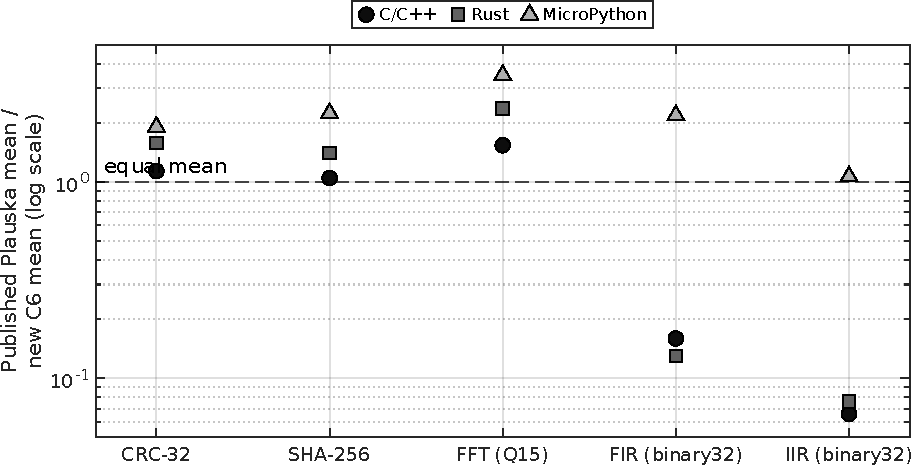
\includegraphics[width=\linewidth]{mode_a_historical_local.pdf}
\caption{Published Plauska mean divided by new physical C6 mean at the largest common input (log scale). Sources are different experiments; ratios are descriptive.}
\label{fig:historical}
\end{figure}

Within C6, ordering also varies (\cref{fig:language}). CRC medians are 104\,\us for C++ and 72\,\us for Rust (Rust/C++ 0.692). SHA gives 670 and 711\,\us (1.061). FFT gives 1185.562 and 1493.750\,\us (1.260). FIR gives 188774 and 186340\,\us (0.987), while IIR gives 3268 and 3277.5\,\us (1.003). FIR/IIR are therefore near-parity observations, not a language ranking. MicroPython is 22--890$\times$ C++ locally, but interpreter generation, numeric objects, SDK, and implementation details preclude an architectural reading.

\begin{figure}[!htbp]
\centering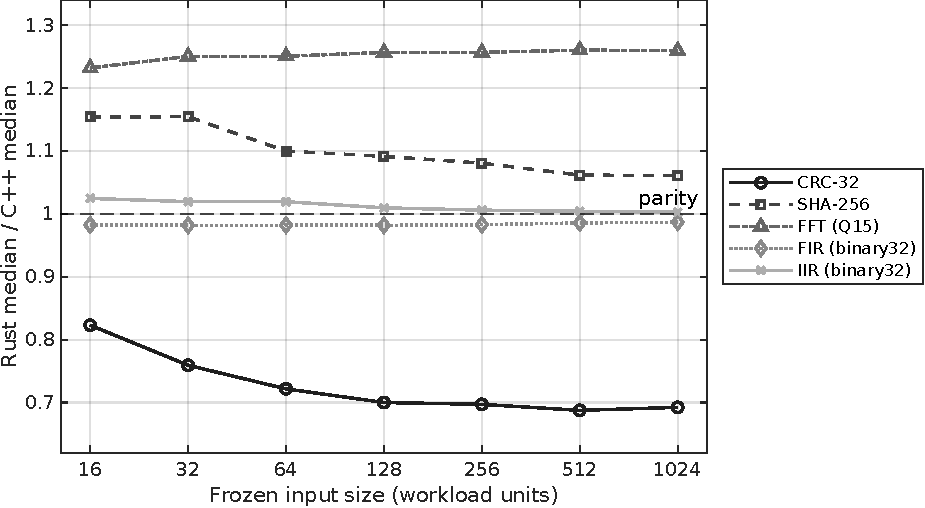
\includegraphics[width=\linewidth]{mode_a_rust_cpp.pdf}
\caption{Within-C6 Mode A Rust/C++ median ratios for nonzero frozen sizes. Size 0 remains in repository evidence but is omitted here because it primarily exposes fixed/timer overhead. Units and work differ by workload; parity is not an equivalence test.}
\label{fig:language}
\end{figure}

Largest-input within-acquisition variation is small for most native groups (for example CRC C++ mean 103.69\,\us, SD 0.884\,\us; FFT C++ mean 1185.568\,\us, SD 0.050\,\us), but says nothing about between-board or between-session uncertainty.

\section{Generated-Code Results}
The disassemblies expose several differences that timing alone cannot locate. We examine exact C6 builds and matched reconstructions separately; neither supplies a dynamic instruction count or a timing breakdown.
\subsection{Integer and fixed-point kernels}
Matched CRC loops expose address formation. Xtensa uses a scaled add while RV32IMAC synthesizes it; both excerpts are copied verbatim from the matched disassemblies under \path{artifacts/assembly/crc32/cpp/}:
\begin{lstlisting}[caption={Matched CRC table addressing; static reconstruction only.}]
# matched Xtensa
addx4 a8, a8, a4
l32i.n a8, a8, 0
# matched RV32IMAC
slli a5,a5,0x2
add  a5,a5,a2
lw   a5,0(a5)
\end{lstlisting}
Matched SHA rotate idioms use Xtensa \texttt{ssai/src} versus RV32IMAC shifts and ORs. Exact Rust SHA also retains more storage/control structure than C++. These observations reveal different lowering, but no dynamic instruction count or cycle contribution.

For Q15 FFT, both targets emit scalar multiplies and shifts. No Xtensa DSP/MAC or zero-overhead-loop instruction appeared in the matched artifact. Safe Rust retains five panic references and larger control structure. The absence is a property of this binary, not evidence that Xtensa lacks such facilities.

\newpage
\subsection{Binary32 kernels and recurrence}
Exact C6 FIR contains two \texttt{\_\_mulsf3} and two \texttt{\_\_addsf3} static call sites; IIR contains five \texttt{\_\_mulsf3}, two \texttt{\_\_addsf3}, and two \texttt{\_\_subsf3}. Because the selected target has no hardware floating-point extension, binary32 arithmetic is lowered to compiler-runtime software floating-point routines \citep{gccSoftFloat1420}. Matched Xtensa FIR emits \texttt{madd.s}; matched IIR emits \texttt{mul.s}, \texttt{madd.s}, and \texttt{msub.s}. Verbatim excerpts are copied from the preserved disassemblies under \path{artifacts/builds/} and \path{artifacts/static/}:
\begin{lstlisting}[caption={Floating-point lowering, copied from the preserved disassemblies under \texttt{artifacts/builds/} and \texttt{artifacts/static/}. Call-site counts are static; reconstructed Xtensa code was not timed.}]
# exact C6 RV32IMAC
42008f0c: jalr -1184(ra) # <__mulsf3>
42008f18: jalr -1308(ra) # <__addsf3>
42008eb6: jalr -1082(ra) # <__subsf3>
# matched Xtensa reconstruction
43: madd.s f0, f2, f1
19: msub.s f1, f2, f0
\end{lstlisting}
The two strategies are not numerically equivalent in general: Xtensa \texttt{MADD.S} and \texttt{MSUB.S} perform no intermediate rounding (\citealp{cadenceXtensaISASummary} \S8.3.159, \S8.3.197), while the C6 target uses separate routines, so the reconstructed and the measured kernels need not agree bit-for-bit beyond the frozen tolerance. Independent of that numerical question, IIR carries state from one output sample to the next, which constrains cross-sample reordering and lengthens the dependence chain. Compiler scheduling may differ, but the present static evidence cannot quantify its timing effect.

\section{Mode B Results}
\begin{table}[!htbp]
\centering\small
\caption{Selected largest-input Mode B observations. Each B/A ratio uses that language's own Mode A median.}
\label{tab:modeb}
\begin{tabular}{@{}llrr@{}}
\toprule
Workload/profile & Language & Median (\(\mu\)s) & B/A \\
\midrule
CRC GCC -O2 & C/C++ & 78.000 & 0.750 \\
CRC Rust opt-3 & Rust & 77.500 & 1.076 \\
SHA GCC -O2 & C/C++ & 626.000 & 0.934 \\
SHA Rust opt-3 & Rust & 628.000 & 0.883 \\
FFT audited transform & Rust & 1134.250 & 0.759 \\
SHA hardware path & C/C++ & 77.000 & 0.115 \\
\bottomrule
\end{tabular}

\end{table}

Compiler response is not uniform (\cref{tab:modeb}, \cref{fig:compiler}). C++ CRC improves 25.0\%; C++ SHA and FIR improve about 6.6--6.7\%; C++ FFT regresses 4.9\%. Rust SHA improves 11.7\%, whereas Rust CRC regresses 7.6\%. Remaining low-single-percent changes are observations from one acquisition, not general optimizer rankings.

\begin{figure}[!htbp]
\centering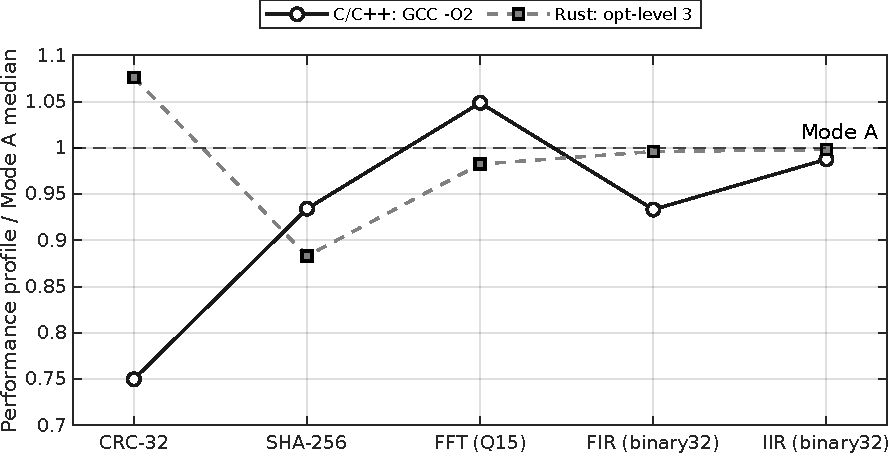
\includegraphics[width=\linewidth]{mode_b_compiler_response.pdf}
\caption{Performance-profile/Mode A median ratios. C++ \texttt{-O2} and Rust opt-level 3 are distinct policies. The clipped detail axis is explicit.}
\label{fig:compiler}
\end{figure}

The SHA hardware profile yields 77\,\us at 1024 bytes: 8.70$\times$ faster than C++ Mode A software and 8.13$\times$ faster than performance-profile software (\cref{fig:sha}). This is a complete SoC/software path, not RISC-V CPU acceleration.

\begin{figure}[!htbp]
\centering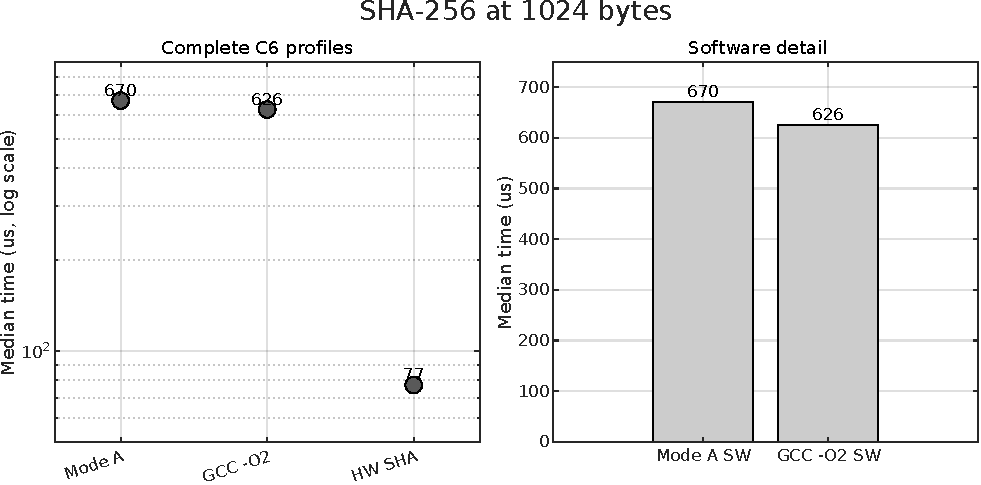
\includegraphics[width=\linewidth]{mode_b_sha_profiles.pdf}
\caption{C6 SHA-256 profiles at 1024 bytes. Left: all profiles (log scale); right: software-only zero-baseline detail.}
\label{fig:sha}
\end{figure}

The remaining Mode B profile is a source-level safety transformation rather than a compiler or peripheral change. Safe Rust performance FFT has 125 static instructions, 398 bytes, 18 branches, five calls, and five panic references. The audited transform has 83 instructions, 246 bytes, eight branches, no calls or panic references (\cref{tab:fft}); its median is 1134.250\,\us, 22.7\% below safe performance Rust. Since the transformation changes the entire kernel, it is not an isolated bounds-check price.

\begin{center}\small
\captionof{table}{Exact C6 Rust FFT generated-kernel profiles.}\label{tab:fft}
\begin{tabular}{@{}llrrrrr@{}}
\toprule
Kernel & Profile & Instr. & Bytes & Branches & Calls & Panic refs. \\
\midrule
FFT & Safe Rust & 125 & 398 & 18 & 5 & 5 \\
FFT & Audited transform & 83 & 246 & 8 & 0 & 0 \\
\bottomrule
\end{tabular}

\end{center}

\section{Discussion}
\paragraph{RQ1.} Target-specific contrasts appear in address formation, rotate lowering, safe control structure, and floating-point lowering. They show how matched workloads present different compiler-visible mechanisms, but not how much each mechanism contributed to Plauska's timings.

\paragraph{RQ2.} No uniform direction emerges. Local native CRC/SHA/FFT means are below published means; FIR/IIR means are above them. Within C6, Rust/C++ ordering varies and FIR/IIR are near parity. MicroPython remains much slower locally while its local means are below published means for all five kernels. Runtime and implementation changes prevent an ISA interpretation.

\paragraph{Best-supported mechanism.} \eclass{Observed}: exact C6 FIR/IIR binaries call software-FP helpers; matched Xtensa artifacts emit FP instructions; optimized C6 artifacts retain helpers; historical/native timing points in the corresponding direction. \eclass{Documented}: C6 is RV32IMAC without standard \texttt{F}, and targets without hardware floating point lower such arithmetic through compiler-runtime software routines \citep{gccSoftFloat1420}; classic ESP32 has configured floating-point facilities. \eclass{Inferred}: distinct FP execution strategies plausibly contribute materially to the historical/local FIR/IIR gap. Neither helper contribution nor pure FP-unit effect is isolated. IIR recurrence is a further plausible constraint, not a quantified cause.

The transformations also affect different parts of the implementation. Compiler profiles change some timings little and move others in opposite directions. The FFT transform changes the generated kernel, while hardware SHA routes the work through a peripheral. Their speedups therefore answer different optimization questions.

\section{Threats to Validity}
\textbf{Identification.} Only C6 was newly measured. Published classic timing, reconstructed Xtensa objects, and exact C6 artifacts are different evidence classes. Equal nominal 160 MHz neither matches microarchitecture nor establishes cycles. Compiler, SDK, runtime, board, memory, and protocol alternatives remain viable.

\textbf{Sampling.} One board and one acquisition sequence per group do not estimate board, day, supply, ambient, or session variation. One hundred repetitions characterize a sequence, not independent hardware replication. Batching and timer quantization remain in raw evidence. A C++ CRC watchdog diagnostic occurred between timed samples; rows stayed unique and correct, but it records scheduler activity outside the timing boundary.

\textbf{Construct.} Elapsed kernel time does not measure IPC, dynamic instructions, cache misses, energy, memory pressure, or application throughput. Static counts do not measure executed paths.

\textbf{Code generation and external validity.} Matched objects were not executed; the accepted Rust CRC ELF is missing. Safe/unchecked FFT changes complete structure. Helper references and recurrence support hypotheses, not latency decomposition. One board and five compact kernels do not represent all Espressif devices, RISC-V/Xtensa implementations, toolchains, languages, or applications.

\section{Reproducibility and Data/Code Availability}
The experimental anchor is commit \texttt{933363b342ac960c0d364b4c6379b1ac884dec9f}; raw evidence is immutable. Analysis-only package v1.0.0, prepared for Zenodo but not publicly deposited, contains 21,600 accepted timing records, hashes, and Python/MATLAB code for statistics, ratios, four figures, and tables. That sealed package retains the preceding report revision; the present editorial revision 1.0.1 has not yet been packaged. Historical aggregates and static metrics are imported, not re-audited. Inputs, kernels, console captures, binaries, and disassembly remain private pending redistribution review; the package cannot repeat correctness tests, firmware builds, hardware runs, or instruction audits. Access boundaries and licenses are detailed in the supplement and package.

\section{Future Work}
A matched physical classic-ESP32 rerun with current toolchains would strengthen platform-generation comparison, though not isolate ISA without further controls. Multiple boards, sessions, randomized profile order, supply/ambient logging, and dynamic counters would support small-effect and mechanism claims. Targeted software-FP controls could quantify helpers and dependence chains; surgical FFT variants could separate checking from induced layout changes. Precise module/chip-rail instrumentation is required for energy. WebAssembly and other languages remain separate future studies \citep{wallentowitz2022wasm,moron2023wasmjit}.

\section{Conclusion}
Revisiting these workloads on C6 gives no uniform performance ordering. Native CRC-32, SHA-256, and FFT means fall below the historical means, while FIR and IIR go in the other direction; the local Rust/C++ ordering also changes with the kernel. Software floating-point calls in exact C6 FIR/IIR binaries, alongside floating-point instructions in reconstructed Xtensa objects, offer the clearest code-level explanation to investigate next. The present evidence does not measure their share of the timing gap.

The optimization results point to distinct choices: a compiler profile, an audited source transformation, and a peripheral API can change different workloads in different ways. For an application moving to C6, these measurements motivate testing the actual kernel and build configuration. A controlled ISA comparison would require additional experiments; the historical ESP32 results remain context for this one-board study.

\bibliographystyle{plainnat}
\begingroup\scriptsize\setlength{\bibsep}{0pt}\bibliography{references}\endgroup
\end{document}
